%% Developing a solution for multimedia home networking chapter
%% author Liu Peng

To fulfill the need of interoperability between devices in home networking,
Tuxera started a project called Streambels. Which aims to solve the
interoperability issue in multimedia home networking. The solution is to make a
combination of most popular solutions into one and link all the resources
and displays in home. 

Since the hardware and networking settings are not easily changeable. And
nowadays smart phone has great CPU power and networking capability. It is well
adopted in people's home and even people's life. It is essential to develop a
mobile application that can be used to control all the multimedia data flow in
home networking. Through one year's development, our team developed an Android
application that can be used to control and connect every multimedia devices in
the home. The application is integrated with a simple media server,
Airplay/DLNA/Chromecast device discovery, and Airplay/DLNA/Chromecast streaming
control point.

\subsection{Architecture overview}
The architecture of the solution is basically a combination of  the most popular
solutions' solutions into one. The whole architecture contains three parts:
discovery, content management and streaming. 

Discovery component is responsible for device discovery which takes advantage of
both Multicast DNS, Simple Service Discovery Protocol. As discussed in
\ref{upnp}, the UPnP service uses Simple Service Discovery Protocol for device
discovery, the application firstly send a M-Search request over UDP to the
IPv4 multicast address 239.255.255.250 and UDP port 1900. Then the application
listen to other devices' response. DIAL devices will return a response with
Application URL header, while the UPnP/DLNA devices will return a message with
a XML body, which gives detailed service URL and description URL. SSDP is used
for both DLNA discovery and DIAL discovery. 

Content management component is responsible for organizing and
navigating multimedia contents which can be found in the home network. In our
solution, this includes both phone's local storage and DLNA digital media
servers that connects to home network. The sources can be used in all of the
three protocols that we support.

Streaming component is responsible for streaming multimedia content to selected
multimedia receivers, such as TVs, wireless speakers, set top boxes etc. In our
solution, since DLNA, AirPlay video/ photo and chromecast all use HTTP streaming
while AirPlay music uses RTSP. Two types of media servers are built inside our
application. 

A simplified version of our implementation is shown in the figure \ref{chart3}
below:
\begin{figure}[htb]
\centering 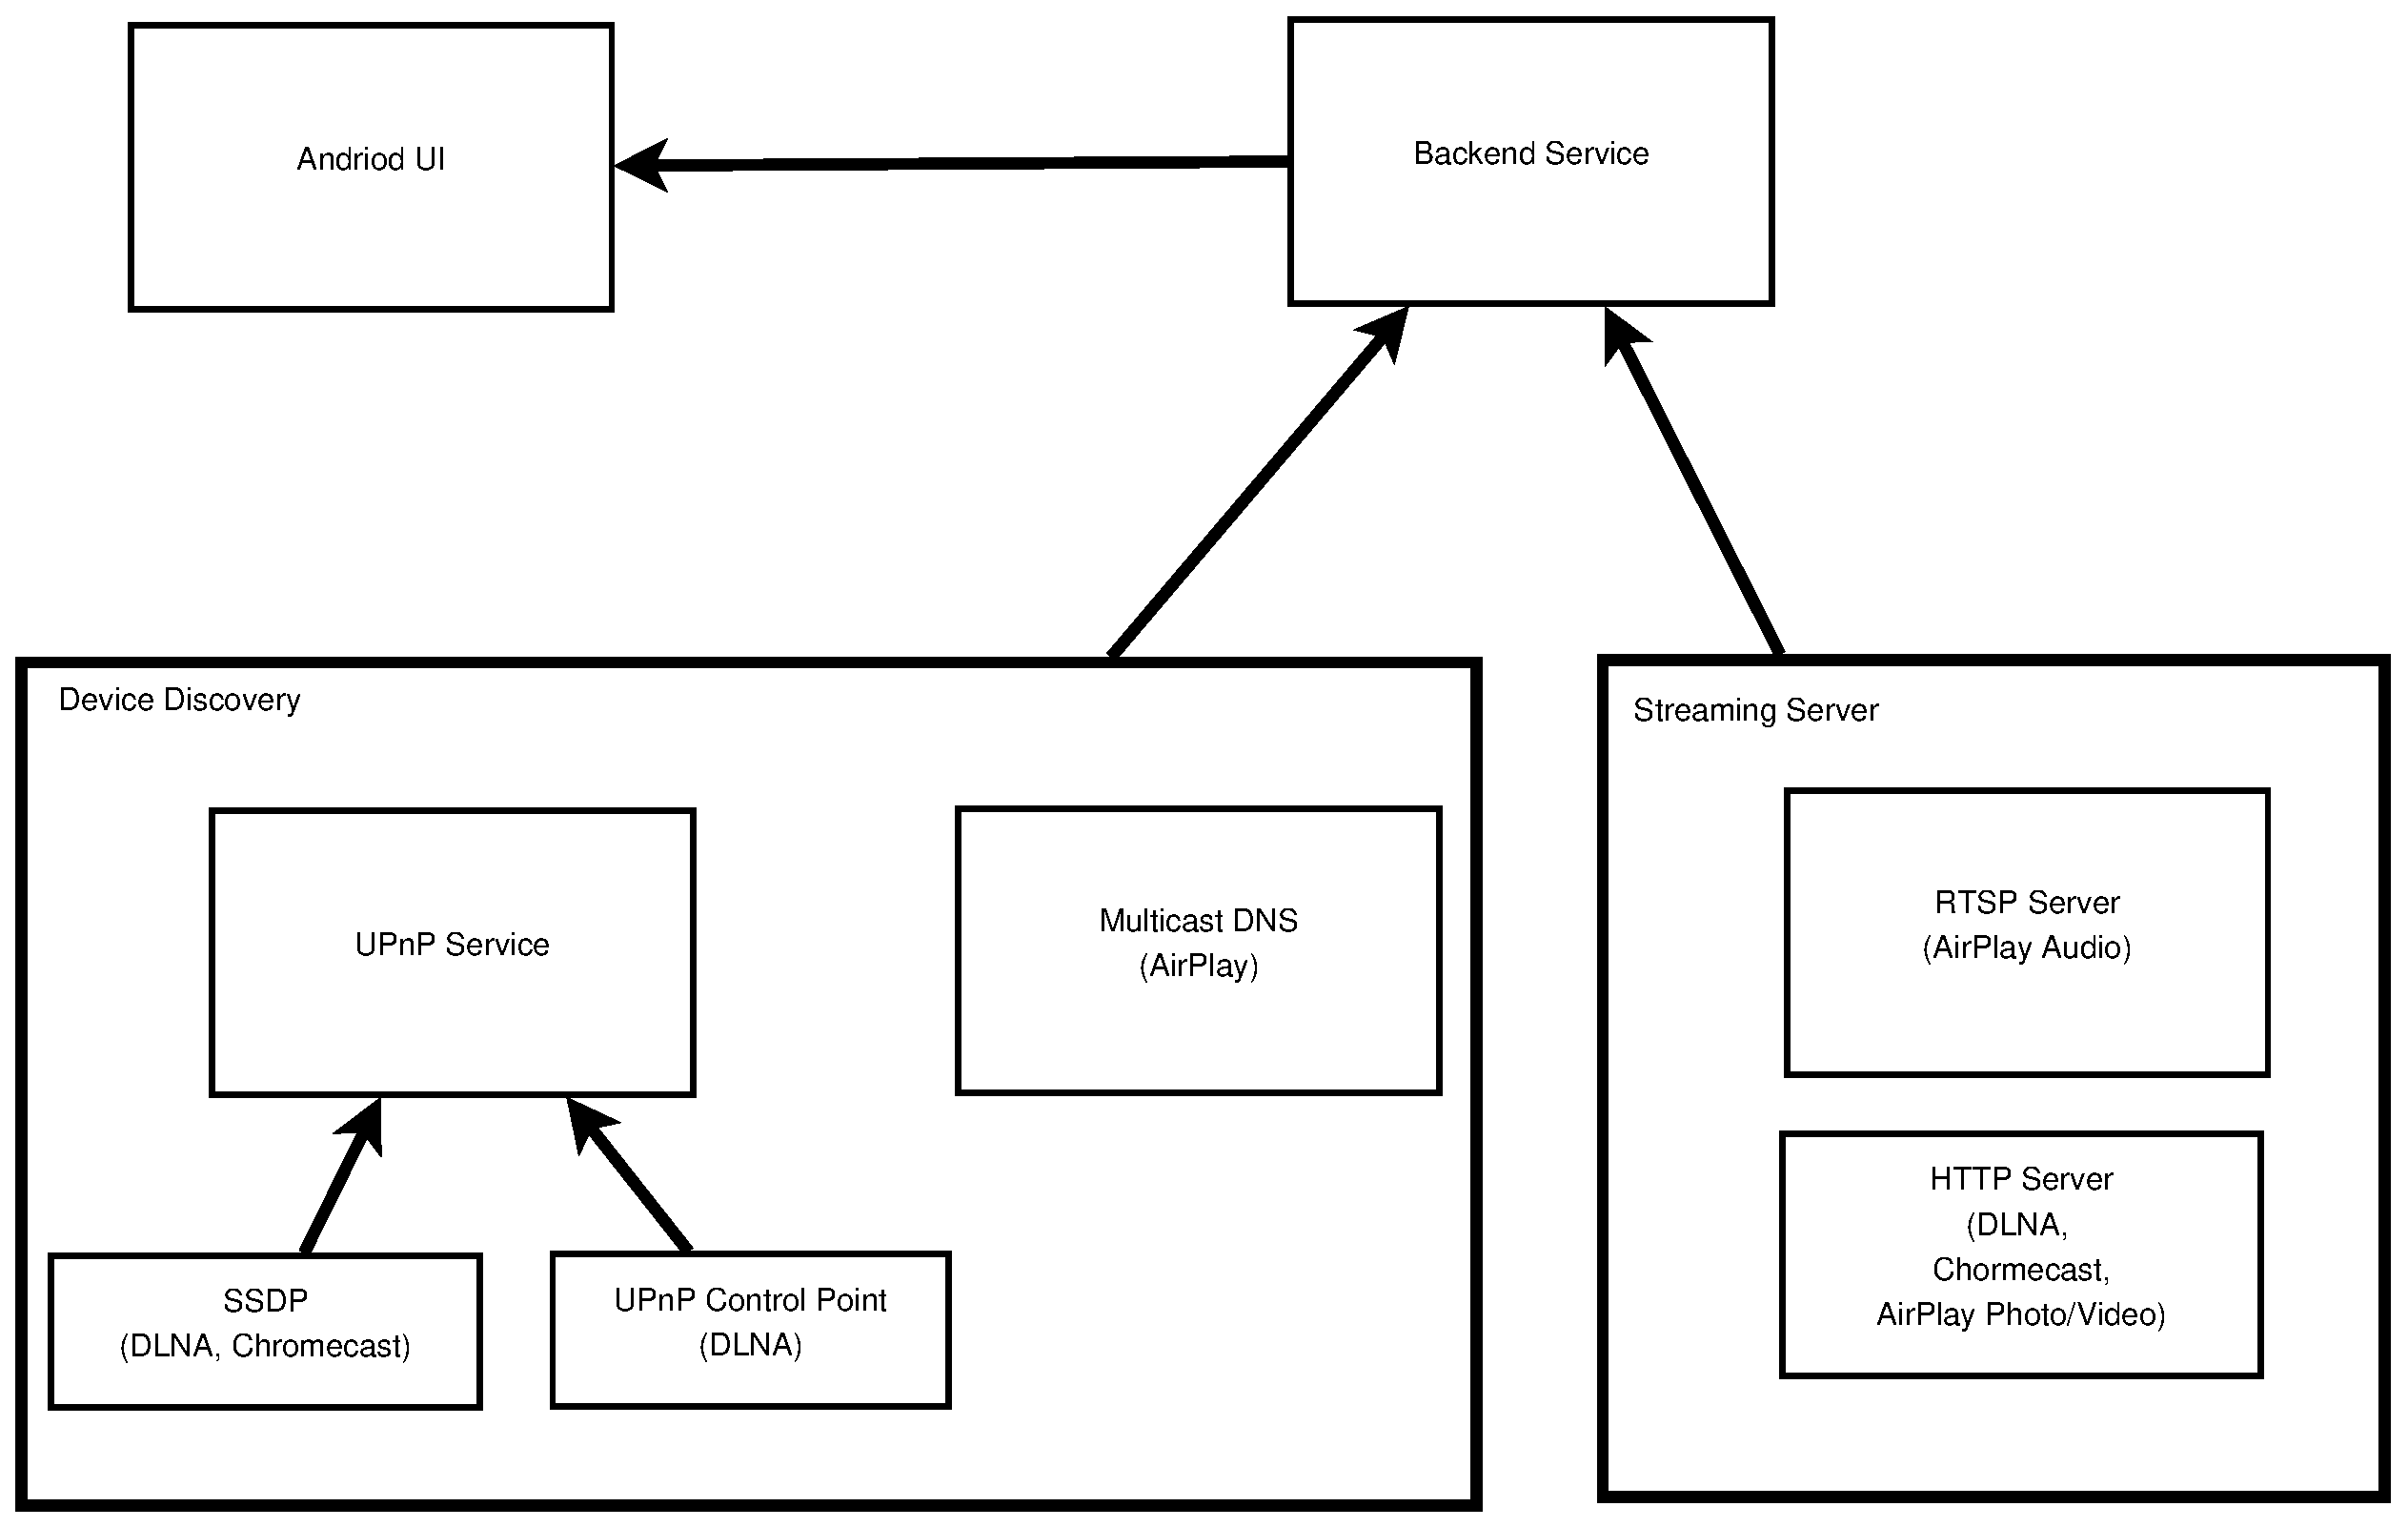
\includegraphics[height=9cm]{charts/chart3}
\caption{Simplified flow chart \label{chart3}}
\end{figure}

In terms of data flow, as described in figure \ref{chart4}, there are three
different types of data flow models: if the streamed content is stored in mobile
phone, a streaming server in the application is used to stream the content from
phone to selected receiver, otherwise, if the content locates on the Internet,
a proxy is used to firstly download the resource stream, add the required
headers by different protocols and then stream the content to selected
receivers, finally, if the streamed content locates in a DLNA Digital Media
Server, the source can be directly used by media renderers, in this case, the
content streaming happened directly from media server to media renderers,
application is only used as a control point in this case.

\begin{figure}[htb]
\centering 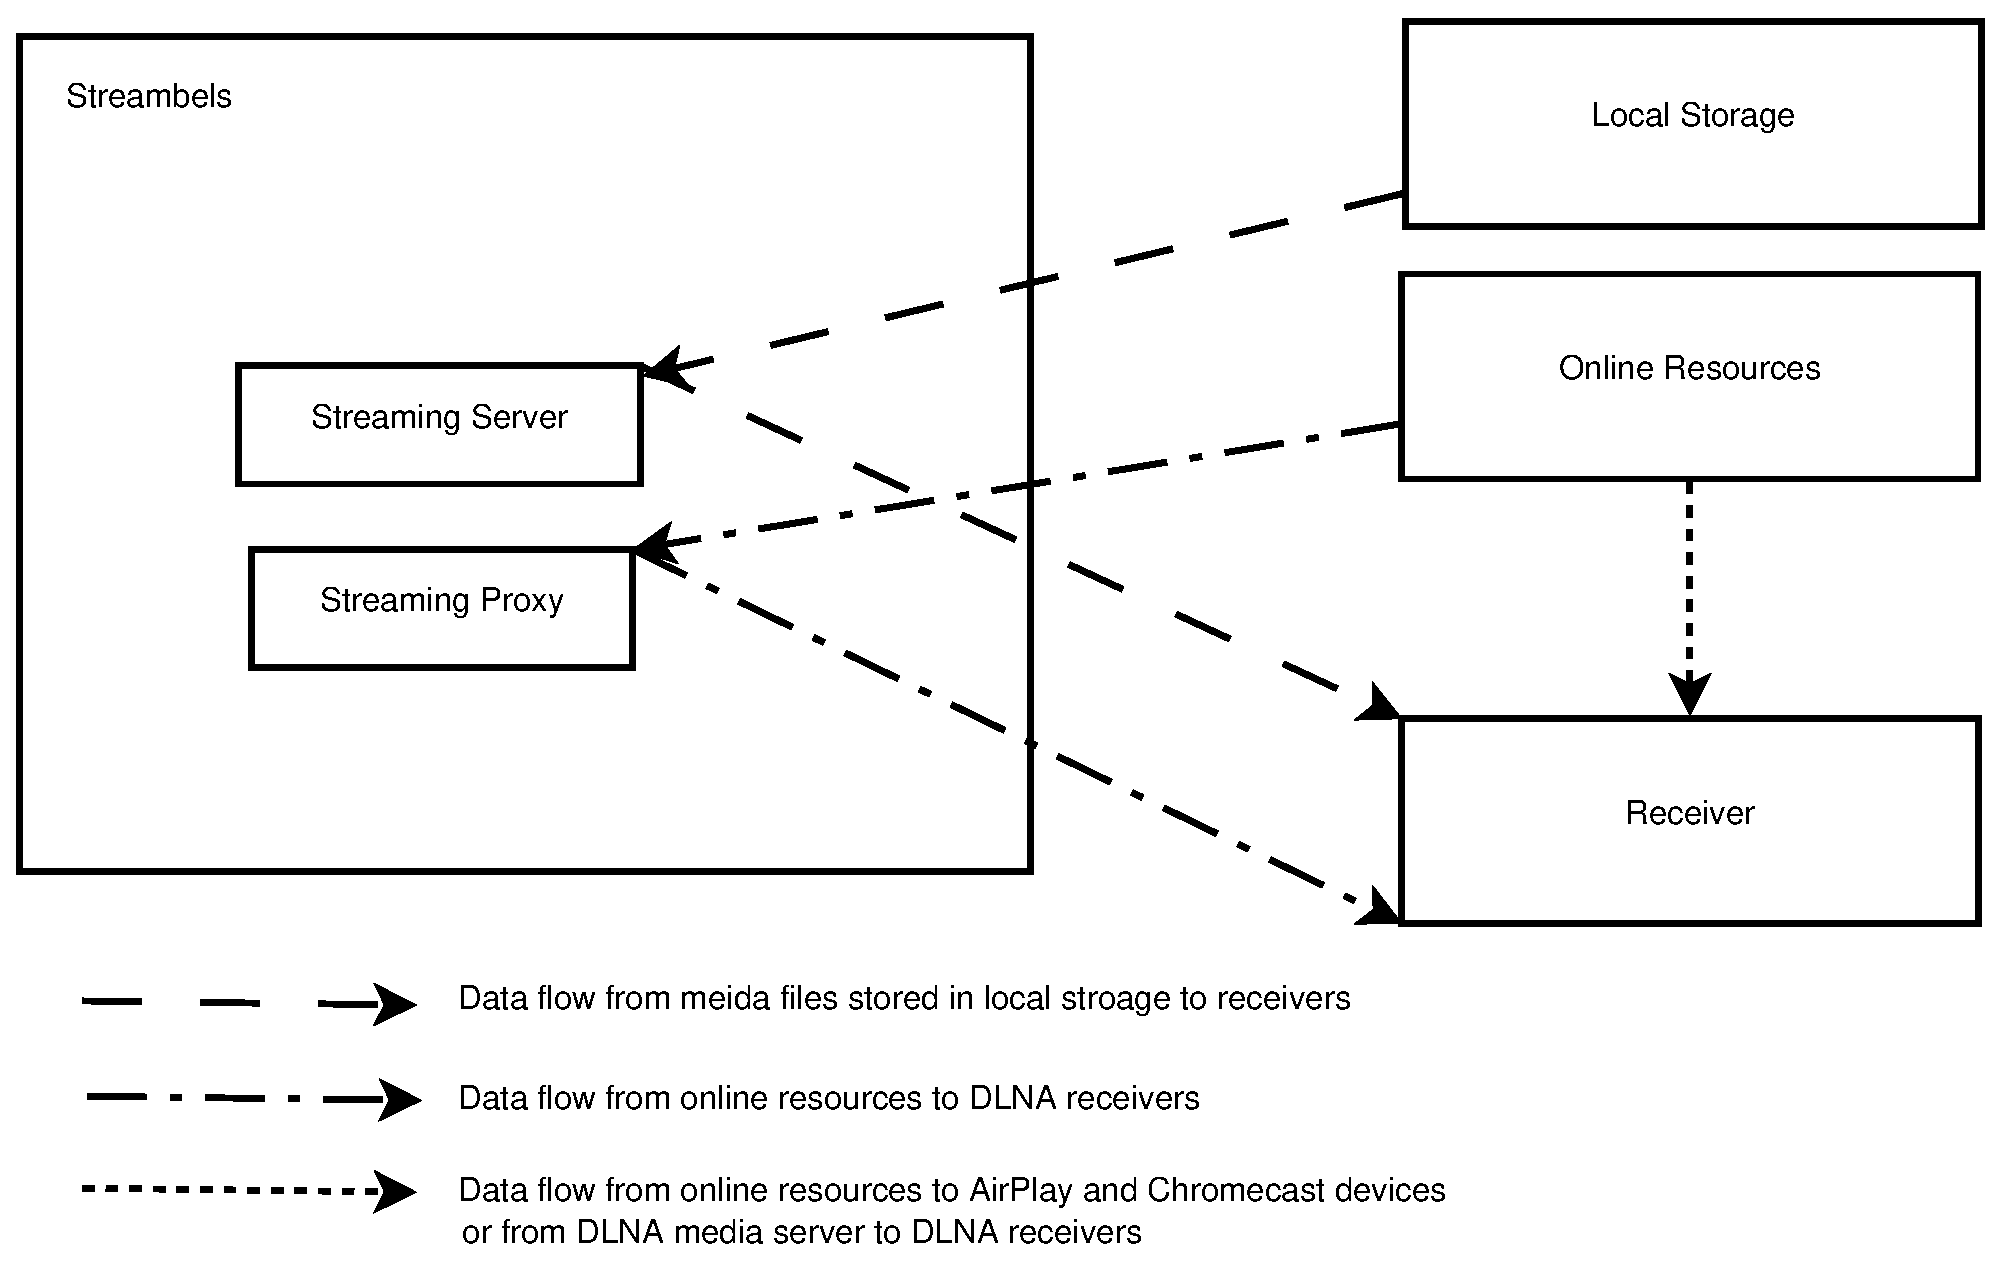
\includegraphics[height=9cm]{charts/data_flow}
\caption{Simplified data flow \label{chart4}}
\end{figure}



\subsection{Features}
As we know that Airplay, DLNA and other standards work differently and have
different features, but according to the previous study, we could combine some
common use cases of both protocols.

The Android application we developed can handle most multimedia devices in 
a typical home networking. Feature list:
\begin{itemize}
\item[--]Firstly the app is a multimedia player, it can play music, photos and videos 
on SD card locally on Android phone
\item[--]It can stream local content to Apple TV, Airport express and Airplay-enabled 
speakers.
\item[--]It can stream local content to DLNA media renderers, which has a huge device 
base.
\item[--]It can stream local content to Chromecast devices.
\item[--]It can browse content from the DLNA media servers, a typical source is a 
Network Attached Storage (NAS). And play the media locally on the Android device.
\item[--]It can browse content from the DLNA media servers and stream it to DLNA media 
renderers.
\item[--]It can browse content from DLNA media servers and stream it to Airplay enabled 
devices using a different protocol.
\item[--]It can proxy online channels' content to DLNA and Airplay enabled devices. 
(Currently YouTube and Facebook videos are supported, but integration to Spotify is still 
in progress).
\end{itemize}

\subsection{Extensibility}
In normal use cases, the data flow can be shown as figure \ref{chart4},
Streambels has embedded a media streaming server for local files and streaming
proxy. By using built-in proxy, Streambels is able to share online resources
from Internet to devices in home networking environment. New services and new
content providers can be easily added by just call the proxy interface.

The proxy system enables a huge extensibility possibility, which connects the
home networking and Internet.

\subsection{Evaluation methodology}
Since the project is targeted to Android market, and is directly used by
end-users, feedback is really important to us for the continuous development. We
used Email for normal communication, user can edit feedback content directly
inside the application, and later content is sent to us by email.

There is no perfect application, so crash sometimes happen, thanks to Google,
the Google will help to collect the crash reports and show it inside developer
console.

Inside Streambels, we also used Google's Analytics API, which give us
great convenience to collect number of users and sessions every day. Other
information like operation system version, application version, active users
helped us to have insights into who are our users and how can we market for more
people in the world.

It is also interesting to see what kind of technologies are most used in their
daily life, thanks to Google's analytics SDK, we can trigger events when user
selected their receivers, so after months of statistics, we can figure out the
most popular standards and most popular online channels that user uses.


